\resetfigpath{intro}
\glsresetall

\chapter{Introduction}
\label{intro}

The medical imaging field has recently witnessed the revolution of \gls{ai}, a broad discipline that is part of computer science, whose aim is to conceptualize human ``intellectual'' tasks, and produce computer programs that can replicate them, thereby allowing to relieve human beings from tedious and repetitive tasks.
From classification to segmentation tasks, \gls{ai} already provides flexible and efficient tools that greatly facilitate the daily practice of clinicians.
In particular, large quantities of \gls{mri} brain scans are now efficiently and accurately processed by \gls{ai} systems that help clinicians in the diagnosis of pathologies \cite{sun19}.
Similarly, surgical instruments can be segmented automatically and accurately in real-time to allow laparoscopic interventions of the abdominal cavity by means of robotic technology, thereby decreasing the invasiveness of traditional methods \cite{davinci}.

Before diving into the underlying intricacies of these systems, we
first wish to give the reader some insights on the genesis of \gls{ai}.
In particular, we describe the two main paradigms that underlie common automated systems, namely the descriptive and predictive analysis paradigms.
In a second section, we explain why one needs large amounts of annotated data to make modern \gls{ai} solutions practical, and how the medical imaging field, in particular, is hindered by this requirement.
Next, we emphasize how the present thesis aims at solving this issue.
Last, we give an overview of the organization of the present thesis.

\section{Descriptive VS. predictive analysis}
\Gls{ml}, a term that denote a sub-category of \gls{ai}, is grounded on the ``learning by example'' paradigm.
Whereas traditional approaches generally consisted in explicitly formalizing and implementing complex tasks as a combination of simpler programmatic instructions,
\gls{ml} rather considers that a flexible system can learn such instructions automatically through repeated experiences.
While both paradigms are in practice complementary, the general trend in many research domains such as computer vision, medical image analysis, computer-assisted intervention in medical applications, shows an increasing shift toward the predictive paradigm, on which \gls{ml} approaches are based.
% Computer vision tasks such as image segmentation and classification were in the early days addressed according to the descriptive analysis paradigm.
% More recently, \gls{ml} approaches, which relie on the predictive analysis paradigm have largely supplanted the latter \cite{omahony19}.
We wish to give the reader some insights on the main differences between these two paradigms.
We first give some generalities, and show, through a concrete example, how the predictive approaches can overcome the limitations of descriptive approaches.

The descriptive approach consists in devising a mathematical model that describes the phenomenon we wish to observe.
This requires to collect a representative dataset of the phenomenon, and identify patterns (or features) that are relevant to the task at hand.
Next, a system is conceived that applies a set of rules to these features, in such a way as to produce the expected outcome.
In practice, finding such set of rules is tedious and error-prone, as the engineer is at risk of missing or misspecifying some important aspects of the phenomenon.
The predictive analysis approach rather considers that the latter component can be obtained by letting a flexible system discover these rules by means of a training procedure.
In particular, predictive analysis considers a model that includes parameterized mathematical operations. The training tasks consists in optimizing these parameters by minimizing an error, taken as a discrepancy measure between the system's output and the expected output.

To better illustrate the differences between the two approaches, let us examine a concrete scenario in which we are interested in elaboring a system that takes as input an image, and must provide at the output an answer to the question ``Does this image contain a car?''.
As a first step, we compute distinctive visual features, assumed to be relevant cues for the task at hand, e.g. large, square-shaped, and homogeneous blobs (assumed to reflect the body of the car), and circular and dark-colored regions (assumed to reflect the wheels).
Both components are characterized by their size, orientation, and location.
A naive approach grounded on the descriptive analysis paradigm, would apply a serie of logical operations such as: (1) Are the wheels located below the body? (2) Are the wheels located at both ends of the body? (3) Is the average size of the wheels inferior to the size of the body?
While these rules seem sensible, they might not cover a number of scenarios, for example: The wheels might be hidden by some objects lying on the scene.

The predictive analysis approach would typically consider a flexible system that defines a number of logical and arithmetic operations between any combination of features.
This system, by being fed a large number of training patterns, i.e. an image with its corresponding correct answer, must discover which logical operation must be applied to which features, which feature to combine, which arithmetic operation to apply, etc..
The task then resolves to inferring by trial-and-error a combination of operations that would best separate the two sets of images.
This is called the ``learning by example'' paradigm.

\section{On the importance of large quantities of annotated data}
\Gls{ml} methods, as the name implies, are built on the ``learning by example'' paradigm.
In their most primitive form, \gls{ml} methods considered feature extraction as a preliminary ad-hoc step, while the design and training of the late-stage predictive model formed another step.
Engineers had to choose for the task at hand which features to choose, which was a tedious and cumbersome task.
More recently, thanks to the technical progress in computing hardware, \gls{dl}, a class of models that elaborate on \gls{nn}, allowed to overcome this limitation.
In essence, \gls{dl} models allow one to optimize both the feature extraction and predictive instances in a joint manner, i.e. through the optimization of a single objective.
This has brought spectacular improvements in performance over traditional methods, making \gls{dl} the de-facto standard in most \gls{ml} fields.
As will be further developped in a next chapter, \gls{dl} models are composed of a concatenation of layers that each perform simple mathematical operations, such as matrix multiplication or convolutions.
The power, flexibility, and hence impressive performance boost of \gls{dl} models, namely comes from the fact that stacking many layers allows to produce rich and abstract features, while the predictive instance can model complex relations.

As showcase application, let us mention the ImageNet Large Scale Visual Recognition Challenge \cite{ILSVRC15}, which consists in classifying natural images into semantic categories such as ``balloon'', ``dog'', etc..
The training dataset contains $150'000$ images, classified into $1000$ categories.
As of today, the state-of-the-art performance uses a \gls{dl} model, in particular a Deep Convolutional Neural Network, which classifies unseen images with an accuracy of $88.6\%$ \cite{tan19}, a performance on par with human capacities.
The model, however, has over $70$ million parameters.
In this scenario, the images has been annotated by many individuals in parallel.

Another example scenario where the above strategy is less practical, is the Brain Tumor Segmentation (BraTS) Challenge \cite{menze15}, which consists in segmenting brain tumors from \gls{mri} scans.
State-of-the-art \gls{dl} models typically account for $\sim 50$ million parameters \cite{chen19}, which are trained using $450$ scans, each containing $\sim 70$ slices (see Fig. \ref{fig:brats}).
A first requirement is that each slice has to be annotated several times to account for disagreements between medical experts.
Second, the tumor are often composed of several distinct regions, e.g. necrotic and non-enhancing tumor, peritumoral edema, and enhancing tumor \cite{akil20}.
All in all, annotating a full MRI scan is estimated to take between 3 and 5 hours of work \cite{kaus01}.

\begin{figure}[!htpb]
  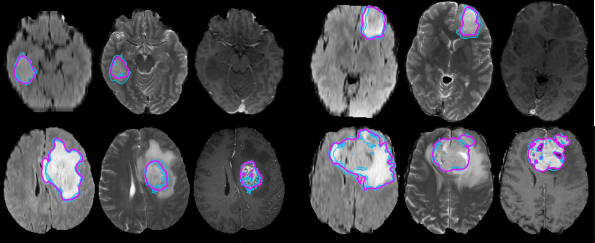
\includegraphics[width=0.99\textwidth]{brats.png}
  \caption{Examples from the BRATS dataset. Annotation of individual experts are in blue, consensus segmentations are in pink. Taken from \cite{menze15}}
  \label{fig:brats}
\end{figure}


\section{Problem definition and thesis statement}

Applying state-of-the-art \gls{dl} methods to segmentation of medical images poses important practical difficulties.
In particular, the task requires a specific medical expertise.
Second, assuming such experts are available and willing to participate to this task, their daily obligations impose a limited time budget.
These two factors largely explain why the field of medical imaging does not benefit from the latest \gls{dl} technologies used in more generic applications \cite{orting19}.
Indeed, the general rule of thumb is: More powerful and flexible model require more training examples.

\textbf{Problem definition}
The present thesis therefore endeavours to address the bottleneck of scarcity of annotated medical images by proposing a fast and intuitive annotation that allows to generate accurate segmentation of objects of interest on a wide variety of medical imaging modalities.

\textbf{Thesis statement}
Generating pixel-wise annotations of medical sequences over a wide range of modalities is greatly facilitated by means of a novel fast and intuitive protocol that relie on sparse point-wise cues, aided by a segmentation framework that relies on \gls{dl} and multi-object tracking.

\section{Organization and Contribution of this Thesis}
The organization of this thesis is now summarized per chapter:

\textbf{Chapter 2} gives an overview of the broad litterature related to the present thesis.
In particular, we first give a state-of-the-art of computer vision methods related to segmentation of images and volumes using sparse annotations.
Next, we review several categories of \gls{ml} methods related to the present scenario, namely \gls{ssl}, \gls{pu}, and \gls{da}.
Last, we add some essential theoretical elements that intervene in the solutions proposed in the present thesis.

\textbf{Chapter 3} gives a detailed description of our fast point-wise annotation protocol.
In particular, the requirements of our annotation protocol is explicitated and justified.
Next, we describe our software solutions, namely a cross-platform and multi-device annotation software, and a web platform with a frontend that allows users to upload annotations, while a backend runs our segmentations algorithms.
We then describe the medical datasets that were used for the evaluation of the proposed segmentation methods, and emphasize how they cover a wide spectrum of real-world use-cases.

\textbf{Chapter 4} contains our first segmentation method that relies on the Expected Exponential loss, optimized using a gradient boosting classifier. The probabilities of unlabeled samples are estimated using label propagation.

\textbf{Chapter 5} gives a thorough study of feature extraction methods, which form an important component of the method presented in the next chapter.
In particular, we first develop an evaluation framework based on a \gls{rf} classifier that operates on superpixels.
As baselines, we implement traditional feature extraction methods, such as \gls{bovw}.
Another baseline considers unsupervised deep feature extraction, where we use a \gls{cnn} trained to classify natural images.
We then implement various methods based on \gls{dl} that integrate motion priors, as well as priors derived from the user-provided point annotations.
Through extensive experiments, we demonstrate the superiority of the \gls{ae} configuration aided by spatial priors.

\textbf{Chapter 6} presents an innovative framework based on multi-object tracking.
Concretely, we formulate our segmentation problem as a maximum a-posteriori problem, where the random variable to optimize is the objectness of superpixels.
Using deep features extracted with the best method of the previous chapter, we train an ensemble of decision trees using a sampling method applicable to the \gls{pu} setup.
Next, simple gaussian kernels provide pairwise similarity measures.
These two models allow to define likelihoods of selecting a superpixel given the user's annotations, and transiting from one frame to the next.
Using the network flow paradigm, we then build a graph that connects superpixels according to spatio-temporal relations.
This chapter covers the content of our first journal article \cite{lejeune18}.

\textbf{Chapter 7} investigates on using a self-supervised clustering method to improve on the feature learning component used in the two previous chapters.
In particular, we speculate that our sequences contain
% TODO: continue this

\textbf{Chapter 8} continues on the same line as the previous chapter by improving on the foreground prediction model.
Instead of using two components, where the first generates deep features, while the second estimates foreground probabilities, we aim at combining the two in an end-to-end fashion.
We leverage a loss function applicable to the \gls{pu} scenario, where the foreground probabilities are inferred by a deep network configured as a predictor.
As the latter loss function requires accurate class priors to render its full potential, we further devise a strategy to estimate the latter in a self-supervised manner.
In particular, our approach consists in setting an initial upper-bound constant value (possibly misspecified) on the prior, and gradually decrease the latter using as evidence the output of the deep network.
Our algorithm relies on the recursive bayesian estimation paradigm.
This chapter covers the content of our second journal article, currently in preparation.

\textbf{Chapter 8} gives a summary of our contributions, provides general discussions on the improvements and limitations of our solutions, and concludes by giving an outline on future works.

%%% Local Variables:
%%% mode: latex
%%% TeX-master: "../../main"
%%% End:
